\section{JPS+}
\label{sec:pre}
%JPS+ is a previously unpublished search strategy
%which we introduce for the 2012 Grid-based Pathfinding Competition.
As we have discussed, jumping from one point to another in the grid
avoids many unnecessary A* queue operations. However, the identification
of these jump points then becomes the bottleneck of the JPS algorithm. 
We therefore propose JPS+: an variant method which reformulates
the input map by replacing each adjacent neighbour of a node with
a jump point that lies in the same relative direction.

\begin{figure}[tb]
       \begin{center}
		   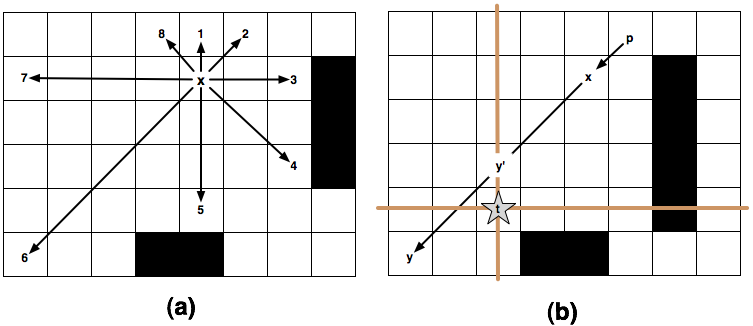
\includegraphics[width=0.95\columnwidth]
			{diagrams/preproc.png}
       \end{center}
	\vspace{-3pt}
       \caption{(a) A jump point is computed in place of each grid neighbour of node $x$.
		the set of neighbours from the grid. (b) In order to reach a jump point $y$ from $x$ it may be
necessary to cross the row or column of the target $t$ (here, both). To make sure we do not jump over 
the target we insert an intermediate successor $y'$ on the row or column of the target (whichever is closest to $x$).}
       \label{fig:preproc}
\end{figure}

\textbf{Reformulation:} 
Figure~\ref{fig:preproc}(a) illustrates our reformulation idea for a 
single node $x$. We simply search for a jump point in the direction
of each grid neighbour of $x$. In JPS, we discard all nodes along a failed
path. By comparison, JPS+ must store the last node along a failed path.
We term such nodes \emph{sterile jump points} and store them only
to guarantee optimality during search; they need never be expanded or even
added to the A* priority queue.
To see why sterile jump nodes are necessary, consider Figure~\ref{fig:preproc}(b).
In this example we reach $x$ from $p$ and try to jump from $x$ to $y$. 
Notice that each such jump may cross the goal or column of the target node
$t$. In JPS the recursion would have terminated at node $y'$ due to a non-failed
straight jump which identifies $t$ as the goal. 
JPS+ simulates this behaviour by explicitly inserting an intermediate node $y'$ 
at the point where the jump to $y$ crosses the column of $t$.
This condition is sufficient to preserve optimality during search. The proof
involves showing that JPS+ simulates exactly the behaviour of JPS. We omit it 
for brevity.

%\textbf{JPS vs JPS+:} 
%Where JPS performs symmetry breaking online, JPS+ differs by breaking
%symmetries during an offline preprocessing step. 
%


